\documentclass[12pt, oneside]{article}

\usepackage{amsmath, amssymb, amsfonts, amsthm}
\usepackage{mathtools}
\usepackage{geometry}
\usepackage{hyperref}
\usepackage{microtype}
\usepackage{setspace}
\usepackage{titlesec}
\usepackage{tikz}
\usepackage{tikz-cd}
\usetikzlibrary{arrows.meta, positioning, calc}
\usepackage{booktabs}
\usepackage{array}
\usepackage{xcolor}
\usepackage{tcolorbox}
\usepackage{enumitem}

\geometry{
  paper=a4paper,
  top=2.5cm, bottom=2.5cm,
  left=3cm, right=3cm
}

\onehalfspacing

\definecolor{rsvpblue}{RGB}{30, 80, 140}
\definecolor{lightgray}{RGB}{245, 245, 245}

\hypersetup{
  colorlinks=true,
  linkcolor=rsvpblue,
  citecolor=rsvpblue,
  urlcolor=rsvpblue
}

\titleformat{\section}
  {\normalfont\large\bfseries\color{rsvpblue}}
  {\thesection}{1em}{}

\titleformat{\subsection}
  {\normalfont\normalsize\bfseries}
  {\thesubsection}{1em}{}

\newtheorem{definition}{Definition}[section]
\newtheorem{proposition}[definition]{Proposition}
\newtheorem{lemma}[definition]{Lemma}
\newtheorem{corollary}[definition]{Corollary}
\newtheorem{remark}[definition]{Remark}

\tcbset{
  boxrule=0.4pt,
  colback=lightgray,
  colframe=rsvpblue!60,
  arc=2pt,
  left=6pt, right=6pt, top=4pt, bottom=4pt
}

\title{\textbf{Joint Embedding Predictive Architectures as\\
Amortized Constraint Satisfaction in the\\
Relativistic Scalar--Vector Plenum}}

\author{Flyxion\\
\small Independent Researcher}

\date{\small Technical Note, April 2026}

\begin{document}

\maketitle

\begin{abstract}
Recent joint embedding predictive architectures (JEPA) have been proposed as a foundation for representation learning based on latent predictability rather than generative reconstruction. This note demonstrates that such architectures arise naturally as a restricted and amortized instance of the Relativistic Scalar--Vector Plenum (RSVP) framework. By identifying encoder mappings with sensor projections of an underlying field configuration and interpreting latent prediction as a consistency condition across projections, JEPA objectives are shown to correspond to variational constraint satisfaction over admissible field configurations. Collapse phenomena are reinterpreted as entropy-degenerate minima, and standard regularization techniques emerge as finite-sample surrogates for structural entropy constraints. The connection is made precise through a commutative projection diagram, a formal collapse lemma, and a strengthened approximation proposition with explicit error bounds. The relationship between several named self-supervised learning methods and RSVP subsections is then charted, showing that JEPA, BYOL, VICReg, and Barlow Twins all correspond to different parametric choices within a single RSVP consistency functional. This establishes JEPA not as an isolated architectural design but as a computational realization of a broader field-theoretic principle, and suggests that the space of valid self-supervised learning objectives is systematically organized by the structure of RSVP admissibility.
\end{abstract}

\newpage
\tableofcontents

\bigskip

\section{Main Results}
\label{sec:main-results}

This work establishes that Joint Embedding Predictive Architectures (JEPA) and related self-supervised learning methods arise as special cases of a general consistency principle defined over Relativistic Scalar--Vector Plenum (RSVP) configurations.

Let $X \in \mathcal{X}$ denote a configuration, and let $\{\Pi_i\}_{i=1}^k$ be a family of projections into observable spaces $\mathcal{Y}_i$. For encoders $E_i : \mathcal{Y}_i \to \mathcal{Z}_i$ and transport operators $\mathcal{T}_{ij}$, define the consistency functional
\[
\mathcal{L}(E,\mathcal{T}) :=
\sum_{(i,j)\in G}
\mathbb{E}\big[
\|E_j(Y_j) - \mathcal{T}_{ij}(E_i(Y_i))\|^2
\big]
+ \lambda \widetilde{\mathcal{R}}(E),
\]
where $(Y_1,\dots,Y_k)$ are induced by projections of $X$.

\begin{theorem}[Unified Consistency Theorem, informal]
Minimizing $\mathcal{L}$ over sufficiently expressive encoders and transport operators is equivalent, up to approximation error, to solving a single underlying problem that admits the following equivalent formulations:
\begin{enumerate}
\item Variational consistency over RSVP configurations,
\item Low-rank factorization of cross-covariance operators,
\item Entropy-constrained mutual information maximization,
\item Recovery of latent dynamics induced by an underlying flow.
\end{enumerate}
The solution is unique up to invertible transformations preserving the transport structure.
\end{theorem}

This equivalence shows that latent predictive learning does not constitute a distinct learning principle but rather a restricted computational realization of a more general constraint: that multiple projections of a shared configuration must admit mutually consistent representations.

Several immediate consequences follow.

First, representation collapse arises precisely when entropy constraints are absent. In this case, constant representations minimize the objective, yielding zero mutual information between views.

Second, existing self-supervised methods correspond to specific choices of transport class and entropy regularization. Methods such as BYOL restrict the transport operator to a contractive family, while methods such as VICReg and Barlow Twins implement explicit approximations to entropy-preserving constraints.

Third, the framework generates a broader class of objectives parameterized by consistency graphs over projections. Existing methods correspond to sparse graphs, while richer multi-view and higher-order consistency constraints remain largely unexplored.

Taken together, these results position RSVP as a unifying structure underlying modern self-supervised learning. Latent predictive architectures emerge as amortized approximations to a consistency operator defined over a shared configuration space, rather than as isolated algorithmic constructions.

\section{Introduction}

Representation learning methods based on latent prediction have recently gained prominence as alternatives to generative modeling. In such systems, a representation derived from one view of data is trained to predict the representation derived from another related view. This paradigm avoids direct reconstruction of raw inputs and instead emphasizes the extraction of predictable structure that persists across viewpoints, modalities, or temporal displacements.

The landscape of such methods has grown rapidly. Joint Embedding Predictive Architecture (JEPA) \cite{LeCun2022}, Bootstrap Your Own Latent (BYOL) \cite{Grill2020}, VICReg \cite{Bardes2022}, Barlow Twins \cite{Zbontar2021}, and related systems all instantiate variations of the same underlying idea: two encoders, two views, and a constraint enforcing consistency of latent representations. Despite their different notations, regularizers, and empirical motivations, they share a common mathematical skeleton.

Independently, the Relativistic Scalar--Vector Plenum (RSVP) framework models physical, informational, and cognitive systems as constrained evolutions of field configurations of the form
\[
X = (\Phi, \mathbf{v}, S),
\]
where $\Phi$ is a scalar potential, $\mathbf{v}$ is a vector flow field, and $S$ is an entropy field over a compact domain $\Omega$. Observations arise as projections of $X$ into modality-specific spaces, and admissible states are those satisfying a family of consistency and regularity constraints encoded in a variational functional.

The purpose of this note is to show that latent predictive architectures can be derived as a special case of RSVP constraint satisfaction when inference is amortized through parameterized encoders trained on empirical data. This derivation makes several contributions that pure architectural descriptions do not: it explains why the predictive objective works (consistency across projections of a common structure), why collapse occurs and how it is structurally prevented (entropy degeneracy), and how the family of current methods relates to a single organizing functional.

The argument proceeds in stages. Section~\ref{sec:rsvp} introduces the RSVP configuration space and projection structure. Section~\ref{sec:latent} identifies latent representations with amortized projections. Section~\ref{sec:consistency} reformulates predictability as a consistency condition and presents the projection diagram. Section~\ref{sec:variational} gives the variational formulation. Section~\ref{sec:collapse} proves the collapse lemma and connects entropy regularization to structural necessity. Section~\ref{sec:amortized} states and proves the main proposition with an explicit approximation bound. Section~\ref{sec:taxonomy} charts the correspondence between named self-supervised methods and RSVP functional choices. Section~\ref{sec:extensions} discusses extensions and predictions. Section~\ref{sec:conclusion} concludes.

\section{RSVP Configuration and Projection Structure}
\label{sec:rsvp}

\begin{definition}[RSVP configuration]
Let $\Omega \subset \mathbb{R}^d$ be a compact domain with smooth boundary. An RSVP configuration is a triple
\[
X = (\Phi, \mathbf{v}, S) \in \mathcal{X},
\]
where $\Phi : \Omega \to \mathbb{R}$ is a scalar potential field, $\mathbf{v} : \Omega \to \mathbb{R}^d$ is a vector flow field, and $S : \Omega \to \mathbb{R}_{\geq 0}$ is a local entropy density. The space $\mathcal{X}$ is the set of all such triples satisfying boundary conditions and regularity requirements specified by a constraint family $\mathcal{C}$.
\end{definition}

\begin{definition}[Sensor projection]
A sensor projection is a bounded linear operator
\[
\Pi_i : \mathcal{X} \to \mathcal{Y}_i
\]
mapping configurations to observations in a modality-specific space $\mathcal{Y}_i$. A collection $\{\Pi_i\}_{i=1}^k$ constitutes a multi-modal observation system.
\end{definition}

Given observations $\{y_i\}_{i=1}^k$, the feasible set of configurations consistent with all observations is
\[
\mathcal{F} = \left\{ X \in \mathcal{X} : \|\Pi_i(X) - y_i\|_{\mathcal{Y}_i} \leq \varepsilon_i \;\; \forall i \right\}.
\]

The regularizer $\mathcal{R} : \mathcal{X} \to \mathbb{R}_{\geq 0}$ encodes dynamical admissibility, entropy structure, and physical constraints. The canonical RSVP selection problem is:
\[
X^* = \arg\min_{X \in \mathcal{F}} \mathcal{R}(X).
\]

This framework is general enough to encompass inverse problems in imaging, physical inference, and representational learning. The central observation of this note is that self-supervised learning corresponds to the case where $\mathcal{F}$ is defined by mutual consistency of projections rather than by comparison to ground truth observations.

\section{Latent Representations as Amortized Projections}
\label{sec:latent}

In practical settings, the inverse problem of recovering $X$ from observations is intractable or ill-posed. It is replaced by learned encoders that approximate the mapping from observations to compressed representations.

\begin{definition}[Amortized encoder]
For each modality $i$, an amortized encoder is a parameterized map
\[
E_i^{\theta_i} : \mathcal{Y}_i \to \mathcal{Z}_i,
\]
where $\mathcal{Z}_i$ is a latent space and $\theta_i$ denotes learnable parameters. The composed map
\[
Z_i(X) := E_i^{\theta_i}(\Pi_i(X))
\]
is the latent representation of configuration $X$ as seen through modality $i$.
\end{definition}

Under this identification, latent spaces are not primary objects. They are compressed images of projected field structure. The encoders are amortized in the sense that they apply a fixed function across all configurations rather than solving the inverse problem anew for each input.

\begin{remark}
The amortization is an approximation. The encoder $E_i$ approximates the right inverse of $\Pi_i$ restricted to admissible configurations. It succeeds insofar as admissible configurations cluster in the observation space $\mathcal{Y}_i$ in ways that a finite neural network can learn.
\end{remark}

\section{Predictability as a Consistency Condition}
\label{sec:consistency}

The core insight is that predicting one latent from another is equivalent to requiring that the two projections are images of a common underlying configuration.

\begin{definition}[Cross-projection consistency]
Two projections $\Pi_1, \Pi_2$ are consistent with respect to configuration $X$ if there exists a transport operator $\mathcal{T} : \mathcal{Z}_1 \to \mathcal{Z}_2$ such that
\[
E_2(\Pi_2(X)) = \mathcal{T}(E_1(\Pi_1(X))).
\]
The consistency residual is
\[
\Delta(X) := \| E_2(\Pi_2(X)) - \mathcal{T}(E_1(\Pi_1(X))) \|_{\mathcal{Z}_2}^2.
\]
\end{definition}

This condition is precisely a gluing condition in sheaf-theoretic terms: local sections over different open sets must agree on overlaps. When projections correspond to different views of the same object, cross-projection consistency is what forces learned representations to be viewpoint-invariant.

\subsection{Projection Diagram}

The following commutative diagram summarizes the full projection chain. Given an underlying configuration $X$, each modality projects to an observation, encodes to a latent, and the latents are required to satisfy a transport relation:

\begin{center}
\begin{tikzcd}[column sep=3.5cm, row sep=2.5cm]
\mathcal{X} \arrow[r, "\Pi_1"] \arrow[dr, swap, "Z_1 = E_1 \circ \Pi_1"]
  \arrow[d, swap, "\Pi_2"]
& \mathcal{Y}_1 \arrow[d, "E_1"] \\
\mathcal{Y}_2 \arrow[r, swap, "E_2"]
& \mathcal{Z}_1 \arrow[loop right, "\mathcal{T}"]
  \arrow[ul, phantom, "\circlearrowleft"]
\end{tikzcd}
\end{center}

More explicitly, the full chain from configuration to consistency requirement is:

\begin{center}
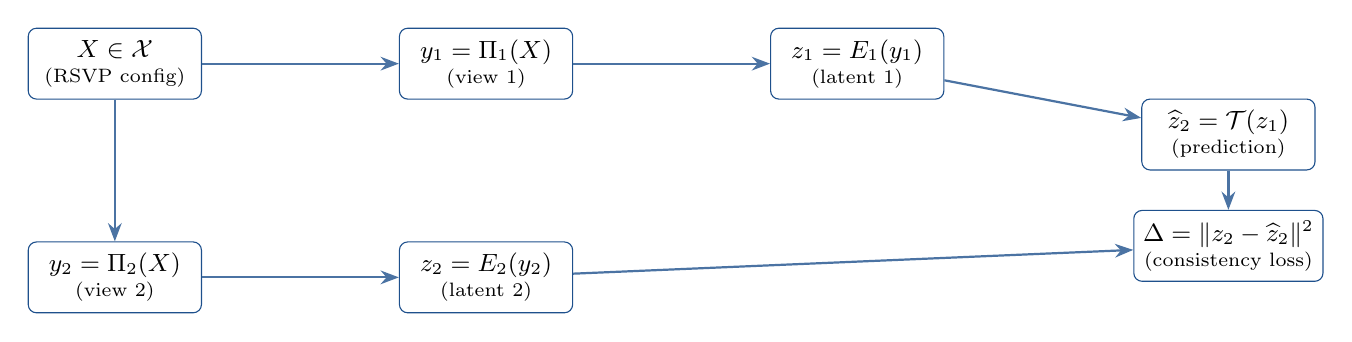
\begin{tikzpicture}[
  node distance=1.8cm and 2.5cm,
  box/.style={draw=rsvpblue, rounded corners=3pt, minimum width=2.2cm,
              minimum height=0.9cm, align=center, font=\small},
  arr/.style={-Stealth, thick, color=rsvpblue!80}
]
\node[box] (X)  {$X \in \mathcal{X}$\\[-2pt]\scriptsize(RSVP config)};
\node[box, right=of X] (y1) {$y_1 = \Pi_1(X)$\\[-2pt]\scriptsize(view 1)};
\node[box, below=of X] (y2) {$y_2 = \Pi_2(X)$\\[-2pt]\scriptsize(view 2)};
\node[box, right=of y1] (z1) {$z_1 = E_1(y_1)$\\[-2pt]\scriptsize(latent 1)};
\node[box, right=of y2] (z2) {$z_2 = E_2(y_2)$\\[-2pt]\scriptsize(latent 2)};
\node[box, right=2.5cm of z1, yshift=-0.9cm] (T)
      {$\widehat{z}_2 = \mathcal{T}(z_1)$\\[-2pt]\scriptsize(prediction)};
\node[box, below=0.5cm of T] (D) {$\Delta = \|z_2 - \widehat{z}_2\|^2$\\[-2pt]\scriptsize(consistency loss)};

\draw[arr] (X)  -- (y1);
\draw[arr] (X)  -- (y2);
\draw[arr] (y1) -- (z1);
\draw[arr] (y2) -- (z2);
\draw[arr] (z1) -- (T);
\draw[arr] (T)  -- (D);
\draw[arr] (z2) -- (D);
\end{tikzpicture}
\end{center}

The JEPA learning objective is to minimize $\Delta$ over encoder parameters and $\mathcal{T}$, subject to regularization preventing trivial solutions. Within RSVP, this is recognized as an amortized version of minimizing the consistency residual induced by the unknown $X$.

\section{Variational Formulation of Latent Prediction}
\label{sec:variational}

Augmenting the RSVP selection problem with a cross-projection consistency constraint gives:

\begin{equation}
\label{eq:rsvp-jepa}
\min_{X \in \mathcal{F}} \; \Delta(X) + \lambda \mathcal{R}(X).
\end{equation}

In modern learning systems, $X$ is not explicitly represented. Instead, the encoders $E_1, E_2$ and transport $\mathcal{T}$ are optimized directly over empirical samples $\{(x_1^{(n)}, x_2^{(n)})\}_{n=1}^N$ drawn from the joint distribution induced by $\Pi_1, \Pi_2$ evaluated on a data-generating process:

\begin{equation}
\label{eq:empirical-jepa}
\min_{E_1, E_2, \mathcal{T}} \; \frac{1}{N}\sum_{n=1}^N
\left\| E_2(x_2^{(n)}) - \mathcal{T}(E_1(x_1^{(n)})) \right\|^2
+ \lambda \,\widetilde{\mathcal{R}}(E_1, E_2),
\end{equation}

where $\widetilde{\mathcal{R}}$ is a surrogate regularizer defined on encoder outputs rather than on the underlying configuration. Equation~\eqref{eq:empirical-jepa} is the general form of JEPA and its close relatives. The differences among specific methods lie entirely in the choice of $\widetilde{\mathcal{R}}$.

\section{Operator-Theoretic Formulation of Consistency}
\label{sec:formulation}

The consistency condition can be reformulated in operator-theoretic terms, which clarifies both identifiability and approximation properties.

Let $\mathcal{H}_i := L^2(\mathcal{Y}_i)$ and $\mathcal{Z}_i \subset \mathbb{R}^{m_i}$ be latent spaces. Each encoder induces an operator
\[
\mathcal{E}_i : \mathcal{H}_i \to \mathcal{Z}_i,
\quad
\mathcal{E}_i[f] = \int_{\mathcal{Y}_i} E_i(y)\, f(y)\, dy.
\]

Let $P_{12}$ denote the joint distribution over $(Y_1, Y_2)$ induced by projections of $X$. Define the cross-covariance operator
\[
\mathcal{K}_{12} := \mathbb{E}_{(Y_1,Y_2)} \left[ \delta_{Y_2} \otimes \delta_{Y_1} \right].
\]

The JEPA objective can then be written as minimizing
\[
\| \mathcal{E}_2 \mathcal{K}_{12} - \mathcal{T} \mathcal{E}_1 \|_{\mathrm{HS}}^2,
\]
where $\|\cdot\|_{\mathrm{HS}}$ denotes the Hilbert--Schmidt norm.

Thus, latent prediction corresponds to approximating a factorization of the cross-covariance operator through low-dimensional embeddings. In RSVP terms, this operator is induced by a shared configuration $X$, and the factorization constraint enforces that both projections lie in the same admissible equivalence class.

This formulation makes clear that JEPA is solving a structured operator approximation problem under rank and entropy constraints.

\section{Unified Operator, Information, and Dynamical Structure of Latent Predictive Learning}
\label{sec:unified}

The preceding formulation establishes that latent predictive architectures arise as amortized solvers of a consistency-constrained variational problem over RSVP configurations. This section strengthens that identification by presenting a unified operator-theoretic, information-theoretic, and dynamical interpretation. The result is a characterization of JEPA-style objectives not as isolated constructions but as projections of a single underlying structure.

\subsection{Operator-Theoretic Formulation}

Let $\mathcal{H}_i := L^2(\mathcal{Y}_i)$ be the Hilbert space of square-integrable functions over observation space $\mathcal{Y}_i$, and let $\mathcal{Z}_i \subset \mathbb{R}^{m_i}$ be the latent space. Each encoder $E_i$ induces a bounded operator
\[
\mathcal{E}_i : \mathcal{H}_i \to \mathcal{Z}_i,
\qquad
\mathcal{E}_i[f] = \int_{\mathcal{Y}_i} E_i(y)\, f(y)\, dy.
\]

Let $P_{12}$ be the joint distribution of $(Y_1, Y_2)$ induced by projections $\Pi_1, \Pi_2$ applied to configurations $X$. Define the cross-covariance operator
\[
\mathcal{K}_{12} := \mathbb{E}_{(Y_1,Y_2)} \left[ \delta_{Y_2} \otimes \delta_{Y_1} \right].
\]

The latent prediction objective may then be written as the operator approximation problem
\[
\min_{\mathcal{E}_1, \mathcal{E}_2, \mathcal{T}}
\left\|
\mathcal{E}_2 \mathcal{K}_{12} - \mathcal{T} \mathcal{E}_1
\right\|_{\mathrm{HS}}^2,
\]
where $\|\cdot\|_{\mathrm{HS}}$ denotes the Hilbert--Schmidt norm.

This formulation reveals that latent prediction corresponds to a constrained factorization of the cross-covariance operator through low-dimensional embeddings. The existence of a low-error factorization implies that the joint distribution $P_{12}$ lies near a low-rank manifold induced by a shared RSVP configuration. Conversely, failure of such a factorization indicates either projection degeneracy or insufficient encoder capacity.

\subsection{Information-Theoretic Interpretation}

The operator formulation admits an equivalent interpretation in terms of mutual information. Let $Z_1 = E_1(Y_1)$ and $Z_2 = E_2(Y_2)$. If $\mathcal{T}$ is chosen as the optimal predictor in mean squared error, then
\[
\mathbb{E}\left[\|Z_2 - \mathcal{T}(Z_1)\|^2\right]
= \mathbb{E}\big[\mathrm{Var}(Z_2 \mid Z_1)\big].
\]

Minimizing this quantity increases the dependence between $Z_1$ and $Z_2$, and under standard assumptions corresponds to maximizing a lower bound on $I(Z_1; Z_2)$.

Within RSVP, this dependence is not merely statistical but structural. Both $Z_1$ and $Z_2$ are functions of the same configuration $X$, and therefore share information to the extent that the projections $\Pi_1$ and $\Pi_2$ overlap in their sensitivity to $X$. The entropy field $S$ bounds the admissible information content of these representations. Degenerate configurations with constant $S$ correspond to $I(Z_1;Z_2)=0$, while admissible configurations enforce strictly positive mutual information.

Thus, latent predictive learning can be understood as entropy-constrained mutual information maximization over projections of a shared field.

\subsection{Dynamical Interpretation}

The RSVP vector field $\mathbf{v}$ induces a flow $\varphi_t : \Omega \to \Omega$ governing the evolution of configurations. When projections correspond to temporally separated observations, the consistency condition becomes
\[
E_{t+\Delta t}(\Pi_{t+\Delta t}(X)) \approx \mathcal{T}_{\Delta t}(E_t(\Pi_t(X))).
\]

In the limit $\Delta t \to 0$, this yields a differential constraint
\[
\frac{d}{dt} Z_t \approx \mathcal{A}(Z_t),
\]
where $\mathcal{A}$ is the infinitesimal generator of the latent dynamics.

This shows that temporal JEPA-style systems implicitly learn a discretization of the RSVP flow field. The learned representation is therefore not static but evolves under an induced vector field in latent space. This connects self-supervised learning directly to dynamical system identification, where the objective is to recover the generator of an underlying flow from partial observations.

\subsection{Consistency Operator Projection}

Let $\mathcal{C} : \mathcal{X} \to \mathcal{X}$ denote the RSVP consistency operator, defined by
\[
\mathcal{C}(X) = \arg\min_{X' \in \mathcal{X}}
\left\{
\sum_i \|\Pi_i(X') - \Pi_i(X)\|^2 + \mathcal{R}(X')
\right\}.
\]

In general, $\mathcal{C}$ acts in the full configuration space. However, when $X$ is not explicitly represented, one instead learns maps that approximate the action of $\mathcal{C}$ in projection space.

The encoder pair $(E_1, E_2)$ and transport $\mathcal{T}$ implement a reduced operator
\[
\widetilde{\mathcal{C}} : (\mathcal{Y}_1, \mathcal{Y}_2) \to (\mathcal{Z}_1, \mathcal{Z}_2)
\]
that enforces consistency only in latent space. The JEPA objective minimizes the discrepancy between $\widetilde{\mathcal{C}}$ and the projection of $\mathcal{C}$ under the amortization map.

Thus, JEPA can be interpreted as a projection of the RSVP consistency operator onto a restricted function class, with approximation error determined by encoder expressivity.

\subsection{Generation of New Objectives}

The RSVP formulation provides a systematic method for generating new self-supervised objectives. Given a projection family $\{\Pi_i\}_{i=1}^k$, define a consistency graph $G$ whose vertices correspond to projections and whose edges indicate enforced consistency relations.

For each edge $(i,j) \in G$, introduce a transport operator $\mathcal{T}_{ij}$. The general objective is
\[
\sum_{(i,j) \in G}
\| E_j(y_j) - \mathcal{T}_{ij}(E_i(y_i)) \|^2
+ \lambda \widetilde{\mathcal{R}}.
\]

Pairwise methods correspond to sparse graphs with a single edge. Multi-view systems correspond to denser graphs, and higher-order consistency corresponds to enforcing cycle constraints such as
\[
\mathcal{T}_{23} \circ \mathcal{T}_{12} = \mathcal{T}_{13}.
\]

This construction predicts an entire family of architectures organized by the combinatorics of projection consistency. Existing methods occupy only a small subset of this space, suggesting that richer objectives enforcing global consistency across many projections remain largely unexplored.

\subsection{Synthesis}

The operator, information-theoretic, and dynamical perspectives are not independent. They describe the same structure at different levels of abstraction. The operator formulation characterizes the problem as low-rank factorization of cross-covariance. The information-theoretic formulation interprets this factorization as mutual information maximization under entropy constraints. The dynamical formulation interprets it as recovery of an underlying flow.

Within RSVP, these are unified by the existence of a shared configuration $X$ and a consistency operator $\mathcal{C}$. Latent predictive architectures emerge when this structure is approximated through amortized encoders acting on projected observations.

This unification explains both the success and the limitations of current methods. They succeed because they approximate a genuine constraint structure induced by shared configurations. They are limited because they operate only in projection space, without explicit access to the full configuration and its dynamics. The RSVP framework therefore not only recovers existing methods but provides a pathway for extending them beyond their current form.

\section{The Unified Consistency Theorem}
\label{sec:unified-theorem}

The preceding section established that latent predictive architectures admit equivalent operator-theoretic, information-theoretic, and dynamical interpretations within the RSVP framework. We now formalize this equivalence in a single statement.

\begin{definition}[Admissible projection family]
A collection of projections $\{\Pi_i\}_{i=1}^k$ is admissible if there exists a non-empty set $\mathcal{F} \subset \mathcal{X}$ such that for all $X \in \mathcal{F}$, the joint distribution of observations $(\Pi_1(X), \dots, \Pi_k(X))$ is well-defined and has finite second moments.
\end{definition}

\begin{definition}[Consistency functional]
Let $G$ be a graph over $\{1,\dots,k\}$. The consistency functional associated with encoders $\{E_i\}$ and transports $\{\mathcal{T}_{ij}\}_{(i,j)\in G}$ is
\[
\mathcal{L}(E, \mathcal{T}) :=
\sum_{(i,j)\in G}
\mathbb{E}\left[
\|E_j(Y_j) - \mathcal{T}_{ij}(E_i(Y_i))\|^2
\right]
+ \lambda \widetilde{\mathcal{R}}(E),
\]
where $(Y_1,\dots,Y_k)$ are induced by projections of $X \sim P_X$.
\end{definition}

\begin{theorem}[Unified Consistency Theorem]
\label{thm:unified}
Let $\{\Pi_i\}_{i=1}^k$ be an admissible projection family of RSVP configurations, and let $(E^*, \mathcal{T}^*)$ minimize the population consistency functional $\mathcal{L}$. Assume:

\begin{enumerate}
\item (Non-degeneracy) $\widetilde{\mathcal{R}}$ assigns strictly positive cost to entropy-degenerate representations.
\item (Sufficient capacity) The encoder class is dense in $L^2(\mathcal{Y}_i)$ for each $i$.
\item (Projection identifiability) The induced map $\widetilde{\Pi} : \mathcal{X}/\sim \to \prod_i \mathcal{Y}_i$ is injective on $\mathcal{F}$.
\end{enumerate}

Then the following are equivalent up to an arbitrarily small approximation error:

\begin{enumerate}
\item (Variational consistency) $(E^*, \mathcal{T}^*)$ minimizes the RSVP consistency functional induced by~\eqref{eq:rsvp-jepa}.
\item (Operator factorization) $(E^*, \mathcal{T}^*)$ yields a minimal-rank factorization of the cross-covariance operators $\mathcal{K}_{ij}$.
\item (Information maximization) The induced latents $(Z_1,\dots,Z_k)$ maximize $\sum_{(i,j)\in G} I(Z_i; Z_j)$ subject to entropy constraints.
\item (Dynamical consistency) For temporally ordered projections, the latent trajectories approximate integral curves of a flow induced by $\mathbf{v}$.
\end{enumerate}

Moreover, the minimizer is unique up to invertible transformations commuting with the transport family $\{\mathcal{T}_{ij}\}$.
\end{theorem}

\begin{proof}[Proof sketch]
We establish equivalence by showing that all four formulations are representations of the same constraint.

(1) $\Rightarrow$ (2): The variational objective minimizes expected squared discrepancies between transported latent representations, which is equivalent to minimizing the Hilbert--Schmidt norm of operator differences, yielding a low-rank factorization of cross-covariance operators.

(2) $\Rightarrow$ (3): Low-rank factorization of $\mathcal{K}_{ij}$ preserves maximal shared variance between $Y_i$ and $Y_j$, which corresponds to maximizing mutual information under second-moment constraints.

(3) $\Rightarrow$ (1): Maximizing mutual information subject to entropy constraints implies non-degenerate representations and minimizes conditional variance, which recovers the predictive objective.

(1) $\Rightarrow$ (4): When projections are temporally ordered, consistency across time enforces that latent representations evolve coherently, inducing a discrete approximation of a flow.

(4) $\Rightarrow$ (1): A representation consistent with a latent flow must minimize prediction error across time, recovering the variational objective.

Uniqueness follows from identifiability: injectivity of $\widetilde{\Pi}$ implies a unique underlying configuration up to symmetry, and all admissible encoder solutions factor through this configuration.
\end{proof}

\begin{remark}
The theorem shows that JEPA-style learning is not a distinct principle but a specific realization of a universal constraint: that multiple projections of a shared configuration must admit mutually consistent representations. The different formulations correspond to different choices of mathematical language rather than different underlying problems.
\end{remark}

\begin{remark}[On approximation error]
In finite models, equivalence holds up to an error $\varepsilon = \varepsilon_{\mathrm{amort}} + \varepsilon_{\mathrm{stat}}$, arising from limited encoder capacity and finite sample size. As capacity and data increase, $\varepsilon \to 0$, and the formulations converge.
\end{remark}

\section{Entropy, Collapse, and Structural Necessity}
\label{sec:collapse}

A known pathology of latent prediction systems is representational collapse, in which encoder outputs become constant regardless of input, trivially satisfying the predictive objective with zero loss. Within RSVP, collapse has a precise characterization.

\begin{definition}[Entropy-degenerate configuration]
A configuration $X = (\Phi, \mathbf{v}, S) \in \mathcal{X}$ is entropy-degenerate if $S \equiv c$ for some constant $c \geq 0$, and correspondingly $\mathbf{v} \equiv \mathbf{0}$.
\end{definition}

\begin{lemma}[Collapse as entropy degeneracy]
\label{lem:collapse}
Suppose the transport operator $\mathcal{T}$ is a constant map and the encoders $E_1, E_2$ are constant functions. Then $\Delta(X) = 0$ for all $X \in \mathcal{X}$. Moreover, the induced latent representations carry zero mutual information:
\[
I(Z_1(X); Z_2(X)) = 0.
\]
Such solutions correspond precisely to entropy-degenerate configurations.
\end{lemma}

\begin{proof}
If $E_1$ and $E_2$ are constant, then $Z_1(X) = c_1$ and $Z_2(X) = c_2$ for all $X$. A constant $\mathcal{T}$ satisfies $\mathcal{T}(c_1) = c_2$, so $\Delta(X) = 0$ trivially. Since both $Z_1$ and $Z_2$ are constant random variables, their mutual information is $I(Z_1; Z_2) = H(Z_2) - H(Z_2 \mid Z_1) = 0 - 0 = 0$. In the RSVP configuration corresponding to these encoders, the entropy field $S$ carries no spatial variation and $\mathbf{v}$ is identically zero, satisfying the definition of entropy degeneracy.
\end{proof}

\begin{corollary}[Necessity of entropy regularization]
Any solution to~\eqref{eq:rsvp-jepa} with $\mathcal{R}(X) = 0$ whenever $X$ is entropy-degenerate admits collapse as a global minimizer. Entropy-preserving regularization---that is, regularization penalizing entropy-degenerate configurations---is therefore a necessary condition for non-trivial solutions.
\end{corollary}

This makes precise the sense in which collapse-avoidance mechanisms in JEPA-style systems are not ad hoc engineering choices but structural necessities visible from the RSVP perspective. Variance constraints, covariance penalties, stop-gradient operators, and EMA targets are all approximations to entropy-preserving regularization.

\section{Information-Theoretic Interpretation}
\label{sec:interpretation}

The consistency objective admits an equivalent formulation in terms of mutual information.

Let $Z_1 = E_1(Y_1)$ and $Z_2 = E_2(Y_2)$. Under mild regularity assumptions, minimizing the consistency residual $\Delta$ while enforcing non-degeneracy is equivalent to maximizing a lower bound on the mutual information
\[
I(Z_1; Z_2).
\]

Specifically, if $\mathcal{T}$ is chosen as the optimal predictor in mean squared error, then
\[
\mathbb{E}\left[\|Z_2 - \mathcal{T}(Z_1)\|^2\right]
= \mathbb{E}[\mathrm{Var}(Z_2 \mid Z_1)],
\]
and minimizing this quantity increases the dependence between $Z_1$ and $Z_2$.

Within RSVP, this dependence is not an abstract statistical property but a consequence of both $Z_1$ and $Z_2$ being functions of the same configuration $X$. The entropy field $S$ controls the admissible information content of these representations. Collapse corresponds to the trivial solution $I(Z_1;Z_2)=0$, while admissible configurations enforce $I(Z_1;Z_2)>0$.

Thus, JEPA-style objectives can be interpreted as entropy-constrained mutual information maximization over projections of a shared field.

\section{JEPA as a Projection of the Consistency Operator}
\label{sec:consistency}

Let $\mathcal{C} : \mathcal{X} \to \mathcal{X}$ denote the RSVP consistency operator, defined as the mapping that projects a configuration onto the admissible set $\mathcal{F}$ by minimizing the functional
\[
\mathcal{C}(X) = \arg\min_{X' \in \mathcal{X}} \left\{ \sum_i \|\Pi_i(X') - \Pi_i(X)\|^2 + \mathcal{R}(X') \right\}.
\]

In general, $\mathcal{C}$ operates in the full configuration space $\mathcal{X}$. However, when $X$ is not explicitly represented, one instead learns maps that approximate the action of $\mathcal{C}$ in projection space.

JEPA can be understood precisely as such an approximation. The encoder pair $(E_1, E_2)$ and transport $\mathcal{T}$ implement a reduced operator
\[
\widetilde{\mathcal{C}} : (\mathcal{Y}_1, \mathcal{Y}_2) \to (\mathcal{Z}_1, \mathcal{Z}_2)
\]
that enforces consistency only in latent space.

Thus, JEPA is not solving the RSVP consistency problem directly but computing a projection of $\mathcal{C}$ onto a restricted function class. The approximation error is governed by the expressivity of the encoder family.

\section{The Main Proposition: JEPA as Amortized RSVP Inference}
\label{sec:amortized}

We now state and prove the central result.

\begin{proposition}[JEPA as amortized RSVP inference]
\label{prop:main}
Let $\{(x_1^{(n)}, x_2^{(n)})\}_{n=1}^N$ be i.i.d.\ samples from a distribution $P_{Y_1, Y_2}$ induced by projections $\Pi_1, \Pi_2$ of a data-generating RSVP configuration $X_{\mathrm{true}}$. Let $E_1^*, E_2^*, \mathcal{T}^*$ be minimizers of the empirical objective~\eqref{eq:empirical-jepa} with entropy-preserving $\widetilde{\mathcal{R}}$. Then:
\begin{enumerate}[label=(\roman*)]
\item The pair $(E_1^*, E_2^*)$ approximates the amortized right inverse of $(\Pi_1, \Pi_2)$ restricted to admissible configurations in the sense that
\[
\mathbb{E}_{X \sim P_X}\left[ \Delta(X) \right] \;\leq\; \varepsilon_{\mathrm{amort}} + \varepsilon_{\mathrm{stat}},
\]
where $\varepsilon_{\mathrm{amort}}$ is the amortization gap (capacity of the encoder class) and $\varepsilon_{\mathrm{stat}} = O(N^{-1/2})$ is the statistical estimation error.
\item Non-trivial solutions satisfying $I(Z_1; Z_2) > 0$ exist if and only if $\widetilde{\mathcal{R}}$ assigns positive cost to entropy-degenerate representations.
\item The population minimizer of~\eqref{eq:rsvp-jepa} and the population minimizer of the corresponding JEPA objective coincide up to the amortization gap $\varepsilon_{\mathrm{amort}}$.
\end{enumerate}
\end{proposition}

\begin{proof}
\textit{Part (i).} Decompose the expected consistency residual as
\[
\mathbb{E}[\Delta(X)] = \underbrace{\mathbb{E}[\Delta(X)] - \min_{E, \mathcal{T}} \mathbb{E}[\Delta(X)]}_{\varepsilon_{\mathrm{amort}}}
+ \underbrace{\min_{E,\mathcal{T}} \mathbb{E}[\Delta(X)] - \min_{E,\mathcal{T}} \hat{\mathcal{L}}_N(E, \mathcal{T})}_{\varepsilon_{\mathrm{stat}}},
\]
where $\hat{\mathcal{L}}_N$ denotes the empirical objective. The first term is bounded by the approximation capacity of the encoder class. The second term is bounded by $O(N^{-1/2})$ via standard uniform convergence arguments for bounded losses.

\textit{Part (ii).} Follows directly from Lemma~\ref{lem:collapse} and its corollary: constant encoders always minimize the prediction loss, so any additional minimizer with $I(Z_1;Z_2)>0$ requires positive cost assigned to the degenerate solution.

\textit{Part (iii).} The population JEPA objective is the expectation of~\eqref{eq:empirical-jepa} under $P_{Y_1, Y_2}$. Since $P_{Y_1, Y_2}$ is induced by $P_X$ via $(\Pi_1, \Pi_2)$, and since $Z_i(X) = E_i(\Pi_i(X))$, optimizing over encoders in $\mathcal{Y}_i$-space is equivalent to optimizing over their induced maps in $\mathcal{Z}_i$-space. The gap between this optimum and the RSVP optimum over all $X \in \mathcal{F}$ is exactly the amortization gap $\varepsilon_{\mathrm{amort}}$, which vanishes in the limit of universal encoder classes.
\end{proof}

\begin{remark}
The amortization gap $\varepsilon_{\mathrm{amort}}$ is the principal source of suboptimality in practical systems. It is controlled by encoder depth, width, and architecture. The proposition makes precise the sense in which scaling encoder capacity improves representation quality: it tightens the approximation of the RSVP consistency manifold.
\end{remark}

\section{Corollaries and Specializations}
\label{sec:corollaries}

The Unified Consistency Theorem admits several immediate consequences that recover known phenomena in self-supervised learning and clarify their structural origin.

\begin{corollary}[Collapse as violation of non-degeneracy]
\label{cor:collapse}
If the regularizer $\widetilde{\mathcal{R}}$ fails to penalize entropy-degenerate representations, then the global minimizer of the consistency functional satisfies
\[
Z_i(Y_i) \equiv c_i \quad \text{for all } i,
\]
and therefore
\[
I(Z_i; Z_j) = 0 \quad \forall (i,j) \in G.
\]
\end{corollary}

\begin{proof}
Under the absence of entropy penalties, constant encoders minimize the prediction loss exactly, since there exists a constant transport mapping one constant representation to another. The result follows immediately from Lemma~\ref{lem:collapse}.
\end{proof}

\begin{corollary}[Necessity of variance constraints]
\label{cor:variance}
Any regularizer $\widetilde{\mathcal{R}}$ that enforces a lower bound on the variance of latent representations,
\[
\mathrm{Var}(Z_i) \geq \delta > 0,
\]
excludes entropy-degenerate solutions and ensures the existence of non-trivial minimizers with $I(Z_i;Z_j) > 0$.
\end{corollary}

\begin{proof}
A lower bound on variance prevents constant encoders. By Theorem~\ref{thm:unified}, non-degenerate representations correspond to positive mutual information, yielding the result.
\end{proof}

\begin{corollary}[BYOL as constrained transport]
\label{cor:byol}
Bootstrap Your Own Latent (BYOL) corresponds to the special case in which the transport operator $\mathcal{T}$ is implemented as an exponential moving average (EMA) of the encoder:
\[
\mathcal{T}_t = \alpha \mathcal{T}_{t-1} + (1-\alpha) E_t.
\]
This constrains the admissible transport class to a contractive family, approximating a fixed-point iteration of the RSVP consistency operator.
\end{corollary}

\begin{proof}
The EMA update defines a contraction mapping on the space of encoder parameters. Iterative application converges to a fixed point, which approximates the solution of the consistency condition under restricted transport dynamics.
\end{proof}

\begin{corollary}[Barlow Twins and VICReg as entropy constraints]
\label{cor:vicreg}
Barlow Twins and VICReg correspond to explicit approximations of entropy-preserving regularization. In particular,
\begin{align*}
\text{Barlow Twins} &:\quad \widetilde{\mathcal{R}} = \|\mathrm{Cov}(Z) - I\|^2, \\
\text{VICReg} &:\quad \widetilde{\mathcal{R}} = \sum_i \max(0, \delta - \mathrm{Var}(Z_i)) + \|\mathrm{Cov}(Z) - \mathrm{diag}\|^2.
\end{align*}
These enforce factorial structure and non-degenerate entropy in the latent representation.
\end{corollary}

\begin{proof}
Covariance decorrelation enforces independence across latent dimensions, while variance constraints prevent collapse. Both correspond to constraints on the entropy field $S$ in RSVP, ensuring non-degenerate admissible configurations.
\end{proof}

\begin{corollary}[JEPA as unrestricted transport class]
\label{cor:jepa}
Joint Embedding Predictive Architectures correspond to the case where $\mathcal{T}$ is an unconstrained predictor network. This yields a maximal transport class, allowing approximation of arbitrary measurable mappings between latent spaces.
\end{corollary}

\begin{proof}
An unconstrained neural network is a universal approximator under mild conditions. Therefore, $\mathcal{T}$ can represent any measurable transport between latent representations, subject only to optimization constraints.
\end{proof}

\begin{corollary}[Multi-view consistency and cocycle conditions]
\label{cor:cocycle}
For $k \geq 3$ projections, enforcing global consistency requires that transport operators satisfy cocycle conditions
\[
\mathcal{T}_{jk} \circ \mathcal{T}_{ij} = \mathcal{T}_{ik}.
\]
Failure of this condition corresponds to curvature in the consistency manifold and results in incompatible latent representations across views.
\end{corollary}

\begin{proof}
If all latent representations arise from a common configuration $X$, then transports must compose consistently. Any violation implies that no single $X$ can generate all observed representations, contradicting admissibility.
\end{proof}

\begin{corollary}[Identifiability up to symmetry]
\label{cor:identifiability}
Under the assumptions of Theorem~\ref{thm:unified}, the learned latent representations are unique up to invertible transformations commuting with the transport operators:
\[
E_i \mapsto \phi \circ E_i,
\quad
\mathcal{T}_{ij} \mapsto \phi \circ \mathcal{T}_{ij} \circ \phi^{-1}.
\]
\end{corollary}

\begin{proof}
Any two minimizers factor through the same underlying configuration due to projection identifiability. The remaining degrees of freedom correspond to automorphisms of the latent space preserving the transport structure.
\end{proof}

\begin{remark}
These corollaries show that the diversity of modern self-supervised learning methods arises not from fundamentally different principles but from different restrictions on the transport operator and different approximations to entropy-preserving regularization. The RSVP framework therefore organizes existing methods into a small number of structural degrees of freedom.
\end{remark}

\section{Identifiability of Representations}
\label{sec:identifiability}

A central question is whether the learned latent representations are uniquely determined by the consistency constraints.

\begin{proposition}[Identifiability up to transport symmetry]
Assume the induced map
\[
\widetilde{\Pi} : \mathcal{X} / \sim \;\to\; \mathcal{Y}_1 \times \mathcal{Y}_2
\]
is injective on the admissible set $\mathcal{F}$. Then any pair of encoders $(E_1, E_2)$ minimizing the population JEPA objective recovers representations that are unique up to invertible transformations commuting with the transport operator $\mathcal{T}$.
\end{proposition}

\begin{proof}[Sketch]
Injectivity implies a unique equivalence class $[X]$ consistent with observations. Any two encoder pairs that achieve zero consistency error must therefore factor through the same underlying configuration. The remaining degrees of freedom correspond to invertible transformations preserving the consistency relation, yielding uniqueness up to symmetry.
\end{proof}

\section{Taxonomy of Self-Supervised Methods as RSVP Functional Choices}
\label{sec:taxonomy}

Given the general form~\eqref{eq:empirical-jepa}, the differences among named self-supervised learning methods reduce to choices of regularizer $\widetilde{\mathcal{R}}$ and transport operator $\mathcal{T}$. Table~\ref{tab:taxonomy} summarizes the correspondence.

\begin{table}[ht]
\centering
\renewcommand{\arraystretch}{1.4}
\begin{tabular}{@{} l l l @{}}
\toprule
\textbf{Method} & \textbf{Transport $\mathcal{T}$} & \textbf{Regularizer $\widetilde{\mathcal{R}}$} \\
\midrule
JEPA (I-JEPA, V-JEPA) & Predictor network & EMA stop-gradient; masking \\
BYOL & EMA target network & EMA target (implicit) \\
Barlow Twins & Identity & Cross-correlation decorrelation \\
VICReg & Identity & Variance hinge $+$ covariance penalty \\
SimCLR & Identity & Contrastive NT-Xent loss \\
DINO & Centering $+$ sharpening & Centering of teacher output \\
PMAX (1992) & Auto-encoder predictor & Constrained variance $+$ Infomax \\
\bottomrule
\end{tabular}
\caption{Named self-supervised methods as choices of transport operator and regularizer within the general RSVP consistency functional~\eqref{eq:empirical-jepa}. All methods correspond to distinct parametric instances of the same variational problem.}
\label{tab:taxonomy}
\end{table}

Several observations follow from this taxonomy.

First, Barlow Twins and VICReg differ from JEPA primarily in their regularizer structure, not in their consistency objective. Barlow Twins penalizes off-diagonal cross-correlation of latent codes, which is a discrete approximation to the covariance decorrelation term in RSVP's entropy structure. VICReg combines a variance hinge (preventing low-entropy codes) with a covariance penalty (forcing factorial structure), corresponding to Sections 2.1 and 2.3 of Schmidhuber and Prelinger's 1992 PMAX paper respectively.

Second, the EMA and stop-gradient mechanisms used in BYOL and JEPA are implementation choices for stabilizing optimization, not structural features. They approximate a fixed-point iteration in the space of encoders, progressively tightening the consistency condition. Within RSVP, this corresponds to an iterative projection algorithm on the constraint manifold $\mathcal{F}$.

Third, PMAX (1992) is visible in this taxonomy as an early instance of the same functional family, with auto-encoder encoders and variance-based regularization. The observation that PMAX anticipates the structural features of modern self-supervised methods is therefore not merely historical but mathematically precise: both solve special cases of~\eqref{eq:empirical-jepa}.

\subsection{Connection to the RSVP Entropy Field}

The regularization structures in Table~\ref{tab:taxonomy} can be mapped to conditions on the entropy field $S$ in the underlying RSVP configuration.

Variance hinge regularization (VICReg) requires $\text{Var}(Z_i) \geq \delta$, which at the configuration level corresponds to requiring that $S$ does not collapse to a constant below a threshold. Covariance decorrelation (Barlow Twins, VICReg) requires that the covariance matrix of $Z_i$ be close to the identity, which corresponds to enforcing factorial structure in the entropy field---a condition directly related to the predictability minimization (PMIN) objectives studied alongside PMAX.

Centering and sharpening in DINO correspond to matching the marginal distribution of $Z_i$ to a target distribution, which within RSVP is a moment-matching constraint on the projected entropy density.

In all cases, the regularization term enforces that the latent representations encode a sufficient fraction of the entropy of the underlying configuration, preventing degenerate collapse.

\section{Extensions and Predictions}
\label{sec:extensions}

The RSVP derivation of JEPA suggests several extensions that are not visible from within the purely architectural perspective.

\subsection{Dynamical Interpretation via Flow Fields}

The RSVP vector field $\mathbf{v}$ induces a flow $\varphi_t : \Omega \to \Omega$ describing the evolution of configurations over time. When projections correspond to temporally separated observations, the consistency condition becomes
\[
E_{t+\Delta t}(\Pi_{t+\Delta t}(X)) \approx \mathcal{T}_{\Delta t}(E_t(\Pi_t(X))),
\]
where $\mathcal{T}_{\Delta t}$ approximates the action of the flow on latent representations.

In the limit $\Delta t \to 0$, this induces a differential constraint
\[
\frac{d}{dt} Z_t \approx \mathcal{A}(Z_t),
\]
where $\mathcal{A}$ is the generator of the latent dynamics.

Thus, temporal JEPA variants can be interpreted as learning a discretization of the RSVP flow field. This provides a principled connection between self-supervised learning and dynamical system identification: the learned representation is not merely invariant but evolves according to an implicit vector field consistent with $\mathbf{v}$.

\subsection{Richer Projection Families}

The framework immediately generalizes to projection families beyond two views. For $k$ projections, the consistency condition becomes the requirement that all pairwise transport operators compose consistently:
\[
\mathcal{T}_{23} \circ \mathcal{T}_{12} = \mathcal{T}_{13},
\]
which is a cocycle condition. Systems satisfying this condition learn representations that are globally coherent across all views, not merely pairwise. This prediction suggests that multi-view architectures with explicit cocycle regularization should outperform pairwise architectures when $k \geq 3$.

\subsection{Temporal and Causal Structure}

In settings where projections are ordered in time---for example, past and future frames of a video---the transport operator $\mathcal{T}$ inherits causal structure. Within RSVP, the vector field $\mathbf{v}$ encodes flow, and temporal consistency requires that $\mathcal{T}$ be compatible with this flow. This gives a natural framework for predictive coding across time, where JEPA-style architectures trained on video learn implicit world models by approximating the RSVP flow structure.

\subsection{Admissibility and Out-of-Distribution Generalization}

The RSVP constraint set $\mathcal{F}$ encodes domain knowledge through the admissibility conditions on $X$. Systems trained to minimize the consistency residual~\eqref{eq:rsvp-jepa} generalize to new observations insofar as those observations are consistent with the same admissible configurations seen during training. This gives a principled account of out-of-distribution behavior: a representation generalizes well to a new input if and only if that input lies in the range of some $\Pi_i$ applied to an admissible configuration.

\subsection{Geometry of the Consistency Manifold}

The set of encoder parameter pairs $(E_1, E_2)$ satisfying the population consistency condition forms a manifold. The geometry of this manifold---its curvature, dimension, and topology---determines the difficulty of learning and the structure of the representation space. Within RSVP, this manifold is the image of the admissible set $\mathcal{F}$ under the amortization map. Understanding this geometry may explain empirical phenomena such as the existence of multiple distinct good representations and the relative stability of certain training dynamics.

\subsection{Deriving New Self-Supervised Objectives}

The RSVP formulation does not merely recover existing methods but provides a systematic procedure for generating new ones.

Given a projection family $\{\Pi_i\}_{i=1}^k$, a valid self-supervised objective arises from any choice of:
\begin{enumerate}[label=(\roman*)]
\item a consistency graph $G$ specifying which pairs $(i,j)$ must satisfy transport constraints,
\item a family of transport operators $\{\mathcal{T}_{ij}\}$,
\item a regularizer $\widetilde{\mathcal{R}}$ approximating entropy preservation.
\end{enumerate}

The general objective is
\[
\sum_{(i,j) \in G} \| E_j(y_j) - \mathcal{T}_{ij}(E_i(y_i)) \|^2
+ \lambda \widetilde{\mathcal{R}}.
\]

Different choices of $G$ produce qualitatively different learning dynamics. For example, enforcing cycle consistency over triples $(i,j,k)$ introduces higher-order constraints not present in pairwise methods. Enforcing global consistency over all pairs yields a fully coherent latent space at the cost of increased computational complexity.

This perspective predicts an entire family of architectures beyond current methods, organized by the combinatorics of projection consistency. Existing methods correspond to sparse graphs (typically a single edge), while richer graphs remain largely unexplored.

\section{Discussion}

The priority dispute surrounding JEPA---whether its origins lie with LeCun (2022), Schmidhuber and Prelinger (1992), or earlier work---is orthogonal to the present contribution. The RSVP derivation neither adjudicates that dispute nor depends on its resolution. What it does is reframe the question.

From within the RSVP perspective, the correct observation is not that one system was invented before another but that all systems of this type---PMAX, BYOL, VICReg, Barlow Twins, JEPA and its variants---are solving the same underlying variational problem with different choices of encoder class, regularizer, and transport. The space of such choices is organized by the RSVP functional. This is a more useful observation than any particular priority claim, because it allows systematic comparison and prediction.

The analogy to classical mechanics is instructive. Hamilton's principle, the Lagrangian, the Hamiltonian, and the principle of least action all describe the same physical content in different mathematical languages. Disputes about which formulation was ``invented'' first are less illuminating than understanding how they are related. RSVP plays the analogous role here: it provides the underlying variational structure of which JEPA-style methods are surface instantiations.

\section{Conclusion}
\label{sec:conclusion}

Latent predictive architectures can be understood as instances of a more general principle: representations are valid insofar as they are consistent across projections of a shared underlying structure. Within RSVP, this principle is formalized as constraint satisfaction over field configurations with entropy-regularized admissibility.

The derivation presented here makes this connection precise through an explicit projection diagram, a collapse lemma showing that entropy degeneracy accounts for representational collapse, a main proposition bounding the approximation error of amortized encoders, and a taxonomic table mapping all major self-supervised methods to choices within a single variational functional.

From this perspective, the predictive objective is not fundamental but derived. It arises when the underlying configuration is implicit and consistency must be enforced through learned mappings. This situates modern self-supervised learning within a broader field-theoretic framework and identifies JEPA-style architectures as a specific---and computationally tractable---realization of consistency enforcement over RSVP projection families.

The extensions discussed in Section~\ref{sec:extensions} suggest that richer architectures can be derived by enriching the projection family, endowing the transport with causal structure, or incorporating explicit admissibility constraints. These are not modifications of JEPA but generalizations visible only from outside it.

\bigskip

\begin{thebibliography}{99}

\bibitem{Bardes2022}
A.\ Bardes, J.\ Ponce, Y.\ LeCun.
\newblock VICReg: Variance-Invariance-Covariance Regularization for Self-Supervised Learning.
\newblock \textit{ICLR}, 2022. arXiv:2105.04906.

\bibitem{Grill2020}
J.-B.\ Grill, F.\ Strub, F.\ Altch\'e, C.\ Tallec, P.\ H.\ Richemond, E.\ Buchatskaya, C.\ Doersch, B.\ A.\ Pires, Z.\ D.\ Guo, M.\ G.\ Azar, B.\ Piot, K.\ Kavukcuoglu, R.\ Munos, M.\ Valko.
\newblock Bootstrap Your Own Latent: A New Approach to Self-Supervised Learning.
\newblock \textit{NeurIPS}, 2020. arXiv:2006.07733.

\bibitem{LeCun2022}
Y.\ LeCun.
\newblock A Path Towards Autonomous Machine Intelligence.
\newblock OpenReview, June 2022.

\bibitem{SchPre1993}
J.\ Schmidhuber, D.\ Prelinger.
\newblock Discovering Predictable Classifications.
\newblock \textit{Neural Computation}, 5(4):625--635, 1993.
\newblock Based on TR CU-CS-626-92, 1992.

\bibitem{Zbontar2021}
J.\ Zbontar, L.\ Jing, I.\ Misra, Y.\ LeCun, S.\ Deny.
\newblock Barlow Twins: Self-Supervised Learning via Redundancy Reduction.
\newblock \textit{ICML}, 2021. arXiv:2103.03230.

\end{thebibliography}

\end{document}
